%************************************************
\chapter{Oblivious Password Authenticated Key Exchange}\label{ch:opake}
%************************************************
In this chapter we present a solution to protect forgetful users from malicious servers.
It is based on the paper ``Oblivious PAKE: Efficient Handling of Password Trials'' \cite{Kiefer13a}, appended in Appendix \ref{paper:opake}.
For in-depth description and thourough formal definitions we refer to Appendix \ref{paper:opake} and concentrate on the high-level concepts in these papers.

We start by recalling the high-level intuition and findings of Appendix \ref{paper:opake}.\footnote{Note that the work in \ref{paper:opake}, while largely rewritten and significantly extended, is based on the M.Sc. Thesis \cite{Kiefer2012}.}
We introduce the notion of \acl{OPAKE} as a solution to the problem of failed login attempts and a general compiler to transform a large class of \ac{PAKE} into \ac{OPAKE} protocols.
\ac{OPAKE} allows a client that shares \emph{one} password with a server to use a \emph{set of passwords} within one \ac{PAKE} session.
It succeeds if and only if one of those input passwords matches the one stored on the server side.
The term \emph{oblivious} is used to emphasize that no information about any password, input by the client, is made available to the server.
Using special processing techniques, our \ac{OPAKE} compiler reaches nearly constant runtime on the server side, independent of the size of the client's password set.
We prove security of the \ac{OPAKE} compiler under standard assumptions using the latest game-based \ac{PAKE} model by \citeauthor{Abdalla2005} (cf. Chapter \ref{ch:pake}), tailored to our needs.
We identify the requirements that \ac{PAKE} protocols must satisfy in order to suit the compiler and give concrete \ac{OPAKE} instantiations.
The compiled protocol is implemented and its performance analysis attests to the practicality of the compiler.
Furthermore, we implement a browser plugin demonstrating how to use \ac{OPAKE} in practice.

The idea of the \ac{OPAKE} compiler is to mix $n$ \ac{PAKE} messages on client side such that the server can extract the ``right'' message using the shared password and reply only to that.
This, however, is a non-trivial problem because \ac{PAKE} messages do not provide information that would allow the server to check locally whether a given password was used in their computation; as this would offer the possibility of offline dictionary attacks.

Our solution for the identification of the ``right'' \ac{PAKE} session is a careful composition of two encoding techniques that were introduced in a different context yet allow us to generically construct \ac{AKE}-secure \ac{OPAKE} protocols from (suitable) \ac{AKE}-secure \ac{PAKE} protocols, preserving constant round complexity and offering nearly constant server load.

Our first building block is \ac{IHME} \cite{Manulis2010,Manulis2011}.
An \ac{IHME} scheme assigns a different index to each given message and encodes the resulting index-message pairs into a single structure from which messages can be recovered on the receiver side using the corresponding indices.
The \ac{IHME} structure hides indices that were used for encoding and therefore all encoded messages must contain enough entropy to prevent dictionary attacks over the index space.
An \ac{IHME} scheme consists of two algorithms \texttt{encode} and \texttt{decode}.
The \texttt{encode} algorithm takes as input a set of index-message pairs $(i_1, m_1),\ldots,(i_n, m_n)$ and outputs a structure $S$ whereas the \texttt{decode} algorithm can extract $m_j$, $j\in[1,n]$ from $S$ using the corresponding index $i_j$.
The corresponding index-hiding property demands that no information about indices $i_j$ is leaked to the adversary that doesn't know the corresponding messages $m_j$ and is defined for messages that are chosen uniformly from the \ac{IHME} message space.
In order to enable encoding of \ac{PAKE} messages using \ac{IHME} with passwords as indices we apply our second building block, namely \emph{admissible encoding} \cite{BonehF01,BrierCIMRT10,pseudorandomSignatures}.
Briefly, a function $F:S\rightarrow R$ is an \emph{$\epsilon$-admissible encoding} for $(S,R)$ with $|S|>|R|$ when for all uniformly distributed $r\in R$, the distribution of the inverse transformation $\cI_F(r)$ is $\epsilon$-statistically indistinguishable from the uniform distribution over $S$.
$\cI_F$ enables us to map \ac{PAKE} messages into the \ac{IHME} message space where necessary.

\noindent\makebox[\textwidth][c]{
\begin{Algorithm}[h!]
		\caption{Client Algorithm}
		\label{alg:clientNext}
		\algsetup{indent=2em}\begin{spacing}{1.3}
{\fontsize{8}{8}\selectfont			\begin{algorithmic}[1]
				\REQUIRE{$\mIn$}
				\ENSURE{$(\mOut,\key)$}
					\STATE $P=\emptyset$%\label{nextc:init}
					\FOR{$i=1\dots n$}
						\IF{$\Pi[i]$ has not finished}
							\STATE $(\mOut',\key)\algout \Pi_{\pwdv[i]}.\mathsf{nextm}(\mIn)$ %\label{nextc:next}
							\STATE $P=P\cup\{(\pwdv[i],\cI_{F^r}(\mOut'))\}$ %\label{nextc:s}
							\STATE $\state[i].\key=\key$%\label{nextc:aggkeys}
						\ELSIF{$\Pi[i]$ has finished $\&\&$\\\hspace*{3em}$\mIn=\PRF_{\Pi[i].\key}(\sid^i_P, 0)$}
							\STATE $\key=\PRF_{\Pi[i].\key}(\sid^i_P,1)$
						\ENDIF
					\ENDFOR
					\IF{$P\not=\emptyset$}
						\STATE $\mOut=\mathsf{IHME}^r.encode(P)$ %\label{nextc:encode}
					\ELSIF{$\key\not\in\cK_{C_\Pi}$}
						\STATE $\key=\bot$ %\label{nextc:bot}
					\ENDIF
				\RETURN $(\mOut,\key)$ %\label{nextc:returnall}
				\vspace*{0.075em}
			\end{algorithmic}}\end{spacing}
\end{Algorithm}}

\noindent
The intuition behind the compiler is to let the client run $n$ \ac{PAKE} sessions, one session for each of the $n$ input passwords $\pwdv$, and apply an index-hiding message encoding on each message-password pair.
The server can apply the shared password $\pwd$ as index to \ac{IHME} to extract the ``right'' \ac{PAKE} message. 
For this message the server computes the next round message of the given \ac{PAKE} protocol and returns the message to the client.
As soon as the underlying \ac{PAKE} protocol terminates, the server generates a confirmation message, which is then used by the client to derive the final session key.
The compiler protocols are given in Algorithm \ref{alg:clientNext} for the client and in Algorithm \ref{alg:serverNext} for the server.
They describe how the next round message is computed using the underlying \ac{PAKE} protocol $\Pi$.
Let $\Pi[i]$ denote the $i$-th instance of $\Pi$ using the $i$-th password $\pwd[i]$, $\mathsf{IHME}^r$ the appropriate IHME scheme for round $r$ and $\cK_\Pi$ the key space of protocol $\Pi$.

\noindent\makebox[\textwidth][c]{
\begin{Algorithm}[H]
		\caption{Server Algorithm}
		\label{alg:serverNext}
		\algsetup{indent=2em}\begin{spacing}{1.3}
{\fontsize{8}{8}\selectfont			\begin{algorithmic}[1]
				\REQUIRE{$\mIn$}
				\ENSURE{$(\mOut,\key)$}
				\IF{$\key=\NULL$ }
					\IF{$\mIn \not= \NULL$}
						\STATE $m\algout \mathsf{IHME}^r.\mathsf{decode}(\pwd,\mIn)$ %\label{nexts:decode}
						\STATE $m'= F^r(m)$
					\ELSE
						\STATE $m'=\mIn$
					\ENDIF
					\STATE $(\mOut,\key)\algout \Pi.\mathsf{nextm}(m')$ %\label{nexts:nextm}
				\ELSIF{$\key\in\cK_\Pi$}
					\STATE $\mOut=\PRF_k(\sid^j_{P'},0)$ %\label{alg:nextsallconfa}
					\STATE $\key\gets\PRF_\key(\sid^j_{P'},1)$ %\label{alg:nextsallconfb}
				\ELSE
					\STATE $(\mOut,\key)=(\emptyset, \bot)$ %\label{nexts:returnallabort}
				\ENDIF
				\RETURN $(\mOut,\key)$ %\label{nexts:returnall}
			\end{algorithmic}}\end{spacing}
\end{Algorithm}}

\begin{figure}[b!]
	\centering
	
\includegraphics[width=\textwidth]{img/LoginBar.png}
	
\includegraphics[width=\textwidth]{img/LoginSuccess.png}
	\caption{Login Browser Bars}\label{fig:loginbar}
\end{figure}
\noindent
To show the practicality of the \ac{OPAKE} compiler we implement it in \verb/C++/, and demonstrate how the compiler can be applied to implementations of the \ac{AKE}-secure, random-oracle-based SPAKE protocol from \cite{Abdalla2005} and the \ac{CRS}-based efficient \ac{PAKE} framework proposed by \citeauthor{Gennaro2008} \cite{Gennaro2008}.
Based on the Firefox extension and PHP server code developed in \cite{MSD13} we implement a Firefox plugin and Apache web server module that allows to use \ac{OPAKE} on a website as a login mechanism.
While the actual user interface does not significantly differ from the implementation in \cite{MSD13}, which is focused on the standard PAKE functionality, the underlying architecture of our \ac{OPAKE} plugin and user experience is new.
We extend the architecture from \cite{MSD13} with a native Firefox plugin and Apache module (implemented in \texttt{C++}) that allows us to use well established cryptographic libraries and our previously described implementation of \ac{OPAKE}.
The first notification bar in Figure \ref{fig:loginbar} displayed on top of the website appears only if the website supports the plugin.
After clicking ``Login'', the actual login window from Figure \ref{fig:loginpopup} is prompted.
The user has the possibility to use the ``plus''-button to create up to $3$ password input fields for his passwords.
When clicking the ``Login''-button the \ac{OPAKE} protocol is executed using the entered passwords on the client side and the stored one on the server side.
The user is successfully logged-in if one of the entered passwords is correct and the browser bar with the green lock is shown (cf. second bar in Figure \ref{fig:loginbar}).

\section{Future Work}
While this work is completed, it provides some follow-up work.
For easier deployment the implementation will be moved towards extension-only code.
Thereby, we have to deal with performance and other JavaScript specific issues.
This should allows seamless installation and operation of the protocols in browsers.
On the theoretical side it may be iteresting to investigate whether \ac{OPAKE} is possible using other buildings block to avoid the increased message size.
%This will be either done using Emscripten compiled C/C++ code and cryptographic libraries or by pure JavaScript implementation.
%We discuss these issues in Chapter \ref{ch:futurework}.

\begin{figure}[htbp]
	\centering
	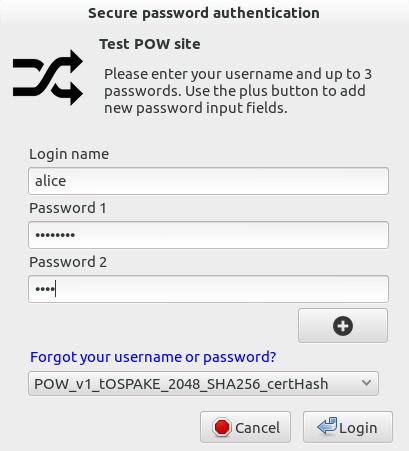
\includegraphics[width=.6\textwidth]{img/LoginPopup.png}
	\caption{Login Popup}\label{fig:loginpopup}
\end{figure}

